\section{Seguridad informática}

\subsection{Ataque Flood}
Implementa y configura ataques basados en ICMP (Ping Flood, Smurf Attack).

\begin{figure}[H]
    \centering
    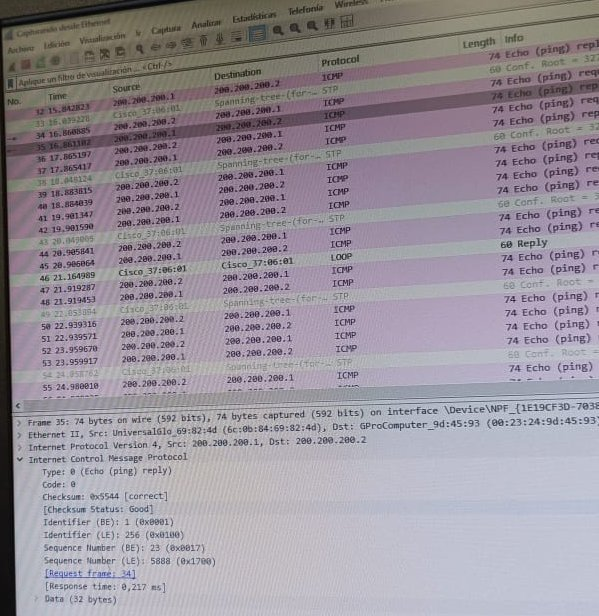
\includegraphics[width=0.75\columnwidth]{punto2/images/1_ping.jpeg}
    \caption{Captura Wireshark, previo ataque.}
\end{figure}

\begin{figure}[H]
    \centering
    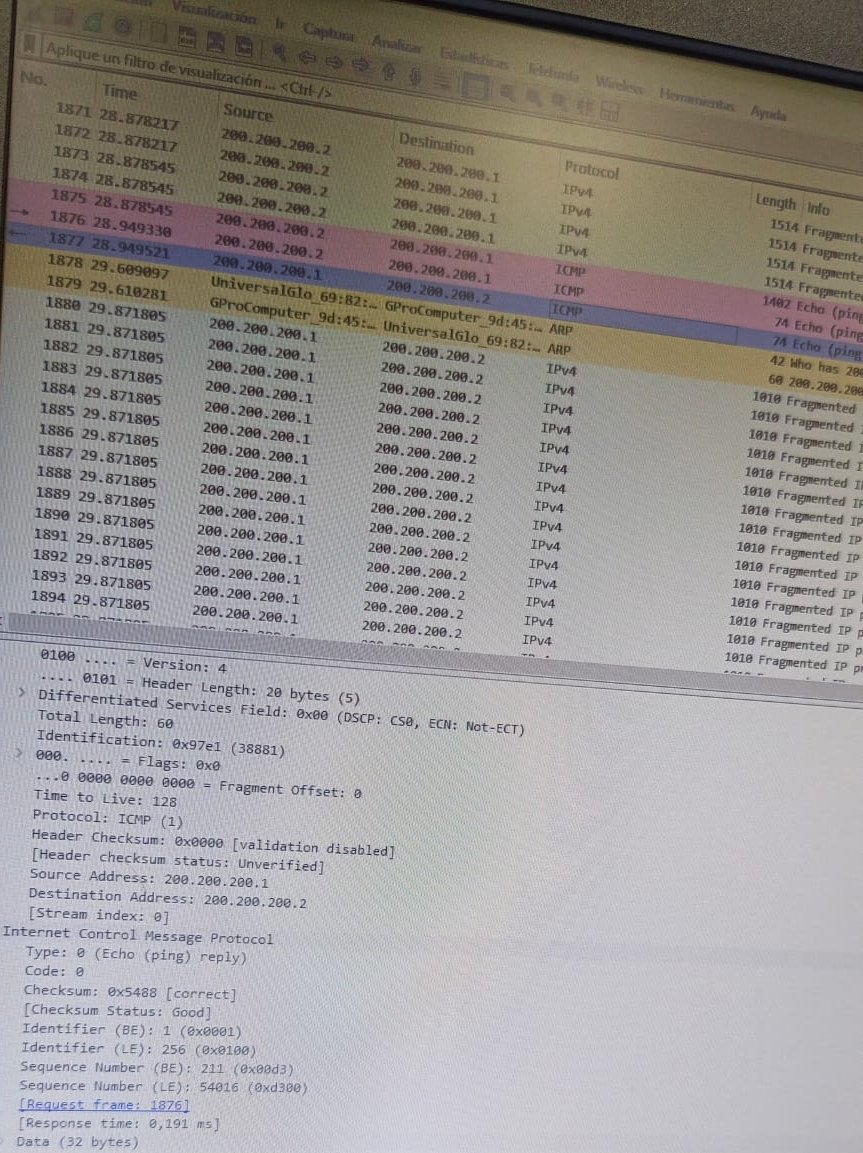
\includegraphics[width=0.75\columnwidth]{punto2/images/2_ping_ataque_flood.jpeg}
    \caption{Ataque flood.}
\end{figure}
\begin{figure}[H]
    \centering
    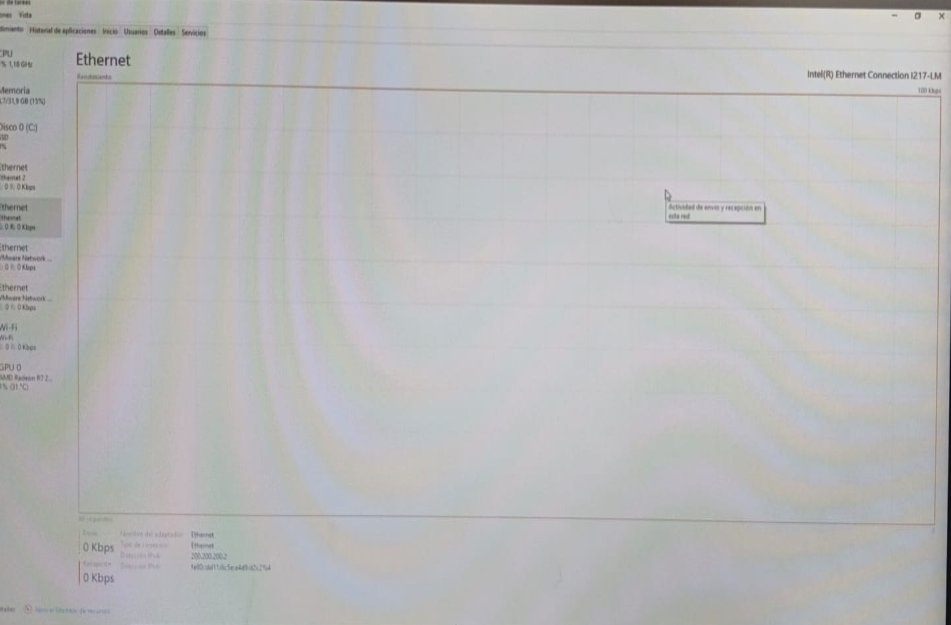
\includegraphics[width=\columnwidth]{punto2/images/3_red_previa.jpeg}
    \caption{Red previo al ataque.}
\end{figure}
\begin{figure}[H]
    \centering
    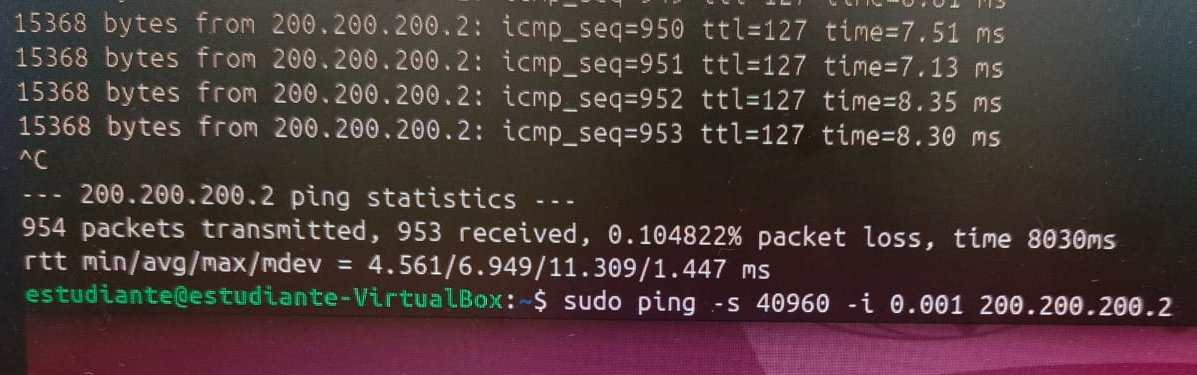
\includegraphics[width=\columnwidth]{punto2/images/4_linux_ataque.jpeg}
    \caption{Ataque desde Linux}
\end{figure}
\begin{figure}[H]
    \centering
    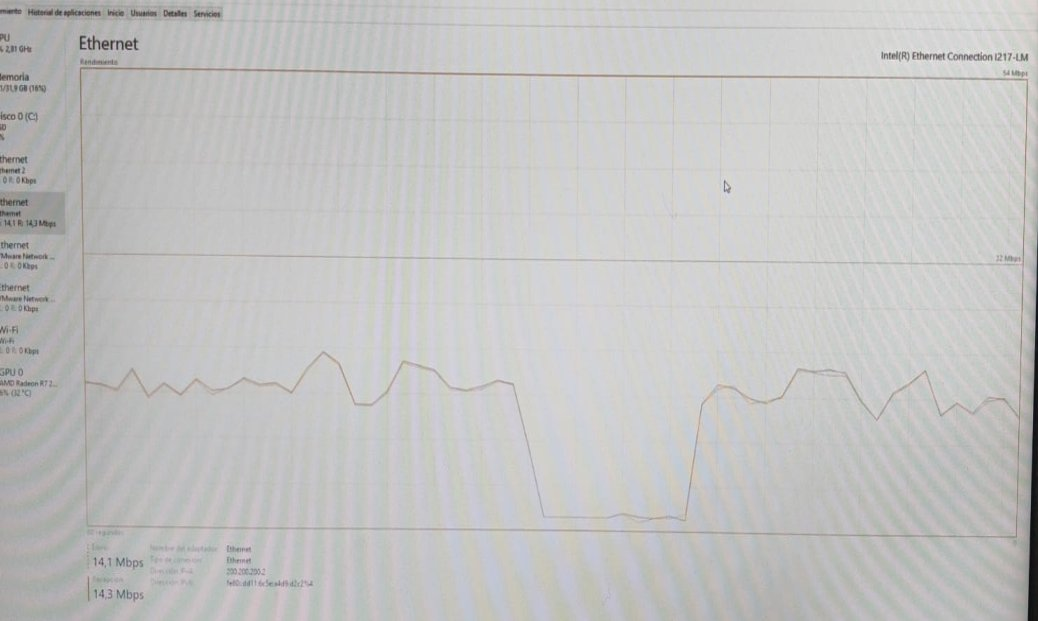
\includegraphics[width=\columnwidth]{punto2/images/5_red_ataque.jpeg}
    \caption{Red en el ataque.}
\end{figure}
\begin{figure}[H]
    \centering
    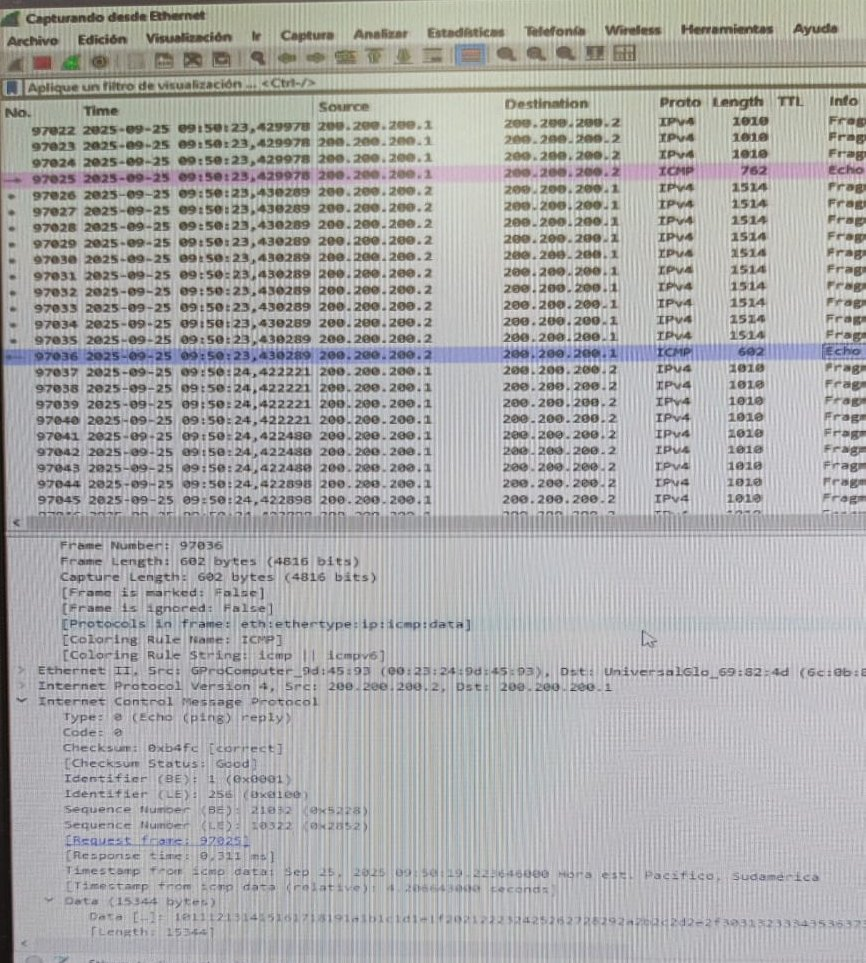
\includegraphics[width=0.75\columnwidth]{punto2/images/6_ws_ataque.jpeg}
    \caption{Captura Wireshark, ataque.}
\end{figure}



% Como afectan las redes LAN IEEE 802.3 y IEEE 802.11 implementadas.

\subsection{Firewall}
Diseñe una regla de firewall que permita ping en LAN (IEEE 802.3 ) pero lo bloquee desde Internet.
%
% Explicar el paso a paso la implementación y las medidas configuradas para mitigar los ataques.

\subsection{Aplicación IA}

Se pidió a la IA generar un script de reglas de firewall en Linux/Windows y luego revisarlo para detectar los ataques mencionados ((Ping Flood, Smurf Attack).

%Explicar el paso a paso la implementación y las medidas configuradas para mitigar los ataques respectivos.
